\section{Bảng đầy đủ}
\label{app:tables}

Mọi bảng trong phụ lục này sinh tự động bởi \texttt{scripts/report/make\_tables.py} từ các file trong \texttt{results/} (xem \texttt{results/README.md}).

\subsection{B3 đầy đủ}

\tabref{tab:b3full} là bảng B3 đầy đủ, 216 ô: 3 mô hình $\times$ 3 mục tiêu $\times$ $\{\lambda = 0, \lambda^*\}$ $\times$ 3 dataset $\times$ 4 horizon, mỗi ô có cả MSE và MAE test.

% Tự động sinh bởi scripts/report/make_tables.py từ results/. KHÔNG SỬA TAY.
{\footnotesize
\begin{longtable}{@{}lrll rr rr rr r@{}}
\toprule
 & & & & \multicolumn{2}{c}{$\lambda = 0$} & \multicolumn{2}{c}{MSE test} & \multicolumn{2}{c}{MAE test} & \\
\cmidrule(lr){5-6}\cmidrule(lr){7-8}\cmidrule(lr){9-10}
Dataset & $H$ & Mô hình & Mục tiêu & MSE & MAE & $\lambda^*_{\mathrm{MSE}}$ & giá trị & $\lambda^*_{\mathrm{MAE}}$ & giá trị & $\delta$ \\
\midrule
\endhead
ETTh1 & 96 & Linear & MSE & 0{,}3702 & 0{,}3915 & 0 & 0{,}3702 & 141{,}3 & 0{,}3915 & -- \\
ETTh1 & 96 & Linear & MAE & 0{,}3653 & 0{,}3833 & 0 & \textbf{0{,}3653} & 0 & \textbf{0{,}3833} & $10^{-6}$ \\
ETTh1 & 96 & Linear & Huber & 0{,}3658 & 0{,}3852 & 3 & 0{,}3658 & 3 & 0{,}3852 & 0{,}538 \\
\addlinespace[2pt]
ETTh1 & 96 & DLinear & MSE & 0{,}3702 & 0{,}3915 & 446{,}7 & 0{,}3698 & 446{,}7 & 0{,}3914 & -- \\
ETTh1 & 96 & DLinear & MAE & 0{,}3653 & 0{,}3833 & 300 & \textbf{0{,}3647} & 100 & \textbf{0{,}3832} & $10^{-6}$ \\
ETTh1 & 96 & DLinear & Huber & 0{,}3658 & 0{,}3852 & 300 & 0{,}3652 & 100 & 0{,}3851 & 0{,}538 \\
\addlinespace[2pt]
ETTh1 & 96 & NLinear & MSE & 0{,}3702 & 0{,}3915 & 1413 & 0{,}3695 & 794{,}3 & 0{,}3913 & -- \\
ETTh1 & 96 & NLinear & MAE & 0{,}3662 & 0{,}3841 & 3000 & \textbf{0{,}3638} & 300 & \textbf{0{,}3839} & $10^{-6}$ \\
ETTh1 & 96 & NLinear & Huber & 0{,}3667 & 0{,}3861 & 1000 & 0{,}3656 & 300 & 0{,}3860 & 0{,}538 \\
\addlinespace[2pt]
ETTh1 & 192 & Linear & MSE & 0{,}4042 & 0{,}4127 & 223{,}9 & 0{,}4040 & 199{,}5 & 0{,}4126 & -- \\
ETTh1 & 192 & Linear & MAE & 0{,}4047 & 0{,}4077 & 1000 & 0{,}4031 & 300 & \textbf{0{,}4074} & $10^{-6}$ \\
ETTh1 & 192 & Linear & Huber & 0{,}4030 & 0{,}4082 & 300 & \textbf{0{,}4025} & 30 & 0{,}4082 & 0{,}582 \\
\addlinespace[2pt]
ETTh1 & 192 & DLinear & MSE & 0{,}4042 & 0{,}4127 & 1000 & 0{,}4036 & 562{,}3 & 0{,}4125 & -- \\
ETTh1 & 192 & DLinear & MAE & 0{,}4047 & 0{,}4077 & 3000 & \textbf{0{,}4014} & 300 & \textbf{0{,}4074} & $10^{-6}$ \\
ETTh1 & 192 & DLinear & Huber & 0{,}4030 & 0{,}4082 & 1000 & 0{,}4017 & 300 & 0{,}4080 & 0{,}582 \\
\addlinespace[2pt]
ETTh1 & 192 & NLinear & MSE & 0{,}4034 & 0{,}4112 & 2512 & 0{,}4027 & 891{,}3 & 0{,}4110 & -- \\
ETTh1 & 192 & NLinear & MAE & 0{,}4064 & 0{,}4080 & $10^{4}$ & 0{,}4026 & 1000 & \textbf{0{,}4075} & $10^{-6}$ \\
ETTh1 & 192 & NLinear & Huber & 0{,}4042 & 0{,}4085 & 3000 & \textbf{0{,}4024} & 300 & 0{,}4084 & 0{,}587 \\
\addlinespace[2pt]
ETTh1 & 336 & Linear & MSE & 0{,}4334 & 0{,}4342 & 1995 & 0{,}4324 & 891{,}3 & 0{,}4340 & -- \\
ETTh1 & 336 & Linear & MAE & 0{,}4372 & 0{,}4283 & $3\cdot 10^{4}$ & 0{,}4302 & 1000 & \textbf{0{,}4275} & $10^{-6}$ \\
ETTh1 & 336 & Linear & Huber & 0{,}4343 & 0{,}4289 & $10^{4}$ & \textbf{0{,}4296} & 1000 & 0{,}4285 & 0{,}621 \\
\addlinespace[2pt]
ETTh1 & 336 & DLinear & MSE & 0{,}4334 & 0{,}4342 & 4467 & 0{,}4317 & 1585 & 0{,}4340 & -- \\
ETTh1 & 336 & DLinear & MAE & 0{,}4372 & 0{,}4283 & $3\cdot 10^{4}$ & 0{,}4296 & 3000 & \textbf{0{,}4272} & $10^{-6}$ \\
ETTh1 & 336 & DLinear & Huber & 0{,}4343 & 0{,}4289 & $10^{4}$ & \textbf{0{,}4290} & 1000 & 0{,}4285 & 0{,}621 \\
\addlinespace[2pt]
ETTh1 & 336 & NLinear & MSE & 0{,}4277 & 0{,}4262 & 8913 & \textbf{0{,}4261} & 1995 & 0{,}4260 & -- \\
ETTh1 & 336 & NLinear & MAE & 0{,}4361 & 0{,}4247 & $3\cdot 10^{4}$ & 0{,}4290 & 3000 & \textbf{0{,}4237} & $10^{-6}$ \\
ETTh1 & 336 & NLinear & Huber & 0{,}4327 & 0{,}4250 & $3\cdot 10^{4}$ & 0{,}4307 & 1000 & 0{,}4246 & 0{,}629 \\
\addlinespace[2pt]
ETTh1 & 720 & Linear & MSE & 0{,}4714 & 0{,}4878 & $1{,}778\cdot 10^{4}$ & 0{,}4701 & 4467 & 0{,}4878 & -- \\
ETTh1 & 720 & Linear & MAE & 0{,}4568 & 0{,}4737 & $3\cdot 10^{4}$ & \textbf{0{,}4553} & $10^{4}$ & \textbf{0{,}4747} & $10^{-6}$ \\
ETTh1 & 720 & Linear & Huber & 0{,}4586 & 0{,}4764 & $3\cdot 10^{4}$ & 0{,}4624 & 3000 & 0{,}4767 & 0{,}709 \\
\addlinespace[2pt]
ETTh1 & 720 & DLinear & MSE & 0{,}4714 & 0{,}4878 & $1{,}778\cdot 10^{4}$ & 0{,}4697 & 5623 & 0{,}4879 & -- \\
ETTh1 & 720 & DLinear & MAE & 0{,}4568 & 0{,}4737 & $3\cdot 10^{4}$ & \textbf{0{,}4549} & $10^{4}$ & \textbf{0{,}4746} & $10^{-6}$ \\
ETTh1 & 720 & DLinear & Huber & 0{,}4586 & 0{,}4764 & $3\cdot 10^{4}$ & 0{,}4620 & 3000 & 0{,}4766 & 0{,}709 \\
\addlinespace[2pt]
ETTh1 & 720 & NLinear & MSE & 0{,}4344 & 0{,}4505 & $1{,}995\cdot 10^{4}$ & 0{,}4329 & 3981 & 0{,}4505 & -- \\
ETTh1 & 720 & NLinear & MAE & 0{,}4318 & 0{,}4445 & $3\cdot 10^{4}$ & \textbf{0{,}4282} & $10^{4}$ & \textbf{0{,}4454} & $10^{-6}$ \\
ETTh1 & 720 & NLinear & Huber & 0{,}4314 & 0{,}4465 & $3\cdot 10^{4}$ & 0{,}4329 & 3000 & 0{,}4468 & 0{,}731 \\
\addlinespace[2pt]
ETTh2 & 96 & Linear & MSE & 0{,}3019 & 0{,}3655 & 1585 & 0{,}3009 & 1413 & 0{,}3649 & -- \\
ETTh2 & 96 & Linear & MAE & 0{,}2789 & 0{,}3342 & 1000 & \textbf{0{,}2779} & 1000 & \textbf{0{,}3334} & $10^{-6}$ \\
ETTh2 & 96 & Linear & Huber & 0{,}2827 & 0{,}3417 & 1000 & 0{,}2818 & 1000 & 0{,}3410 & 0{,}398 \\
\addlinespace[2pt]
ETTh2 & 96 & DLinear & MSE & 0{,}3019 & 0{,}3655 & 1995 & 0{,}3008 & 1585 & 0{,}3649 & -- \\
ETTh2 & 96 & DLinear & MAE & 0{,}2789 & 0{,}3342 & 1000 & \textbf{0{,}2778} & 1000 & \textbf{0{,}3333} & $10^{-6}$ \\
ETTh2 & 96 & DLinear & Huber & 0{,}2827 & 0{,}3417 & 1000 & 0{,}2817 & 1000 & 0{,}3410 & 0{,}398 \\
\addlinespace[2pt]
ETTh2 & 96 & NLinear & MSE & 0{,}2726 & 0{,}3352 & 1778 & \textbf{0{,}2717} & 1585 & 0{,}3342 & -- \\
ETTh2 & 96 & NLinear & MAE & 0{,}2781 & 0{,}3317 & 3000 & 0{,}2764 & 1000 & 0{,}3307 & $10^{-6}$ \\
ETTh2 & 96 & NLinear & Huber & 0{,}2766 & 0{,}3316 & 1000 & 0{,}2756 & 1000 & \textbf{0{,}3306} & 0{,}372 \\
\addlinespace[2pt]
ETTh2 & 192 & Linear & MSE & 0{,}3972 & 0{,}4276 & 1122 & 0{,}3966 & 1122 & 0{,}4273 & -- \\
ETTh2 & 192 & Linear & MAE & 0{,}3541 & 0{,}3861 & 1000 & \textbf{0{,}3531} & 1000 & \textbf{0{,}3855} & $10^{-6}$ \\
ETTh2 & 192 & Linear & Huber & 0{,}3609 & 0{,}3949 & 1000 & 0{,}3600 & 1000 & 0{,}3945 & 0{,}453 \\
\addlinespace[2pt]
ETTh2 & 192 & DLinear & MSE & 0{,}3972 & 0{,}4276 & 1259 & 0{,}3966 & 1259 & 0{,}4273 & -- \\
ETTh2 & 192 & DLinear & MAE & 0{,}3541 & 0{,}3861 & 1000 & \textbf{0{,}3531} & 1000 & \textbf{0{,}3855} & $10^{-6}$ \\
ETTh2 & 192 & DLinear & Huber & 0{,}3609 & 0{,}3949 & 1000 & 0{,}3600 & 1000 & 0{,}3945 & 0{,}453 \\
\addlinespace[2pt]
ETTh2 & 192 & NLinear & MSE & 0{,}3343 & 0{,}3762 & 1585 & \textbf{0{,}3336} & 1585 & 0{,}3754 & -- \\
ETTh2 & 192 & NLinear & MAE & 0{,}3464 & 0{,}3765 & 3000 & 0{,}3447 & 1000 & 0{,}3756 & $10^{-6}$ \\
ETTh2 & 192 & NLinear & Huber & 0{,}3437 & 0{,}3753 & 1000 & 0{,}3427 & 1000 & \textbf{0{,}3744} & 0{,}421 \\
\addlinespace[2pt]
ETTh2 & 336 & Linear & MSE & 0{,}4858 & 0{,}4837 & 1000 & 0{,}4853 & 1000 & 0{,}4835 & -- \\
ETTh2 & 336 & Linear & MAE & 0{,}4116 & 0{,}4301 & 1000 & \textbf{0{,}4106} & 1000 & \textbf{0{,}4296} & $10^{-6}$ \\
ETTh2 & 336 & Linear & Huber & 0{,}4230 & 0{,}4404 & 1000 & 0{,}4220 & 1000 & 0{,}4400 & 0{,}505 \\
\addlinespace[2pt]
ETTh2 & 336 & DLinear & MSE & 0{,}4858 & 0{,}4837 & 1122 & 0{,}4853 & 1122 & 0{,}4835 & -- \\
ETTh2 & 336 & DLinear & MAE & 0{,}4116 & 0{,}4301 & 1000 & \textbf{0{,}4106} & 1000 & \textbf{0{,}4296} & $10^{-6}$ \\
ETTh2 & 336 & DLinear & Huber & 0{,}4230 & 0{,}4404 & 1000 & 0{,}4220 & 1000 & 0{,}4400 & 0{,}505 \\
\addlinespace[2pt]
ETTh2 & 336 & NLinear & MSE & 0{,}3588 & 0{,}4004 & 1585 & \textbf{0{,}3581} & 1413 & \textbf{0{,}3997} & -- \\
ETTh2 & 336 & NLinear & MAE & 0{,}3779 & 0{,}4039 & 3000 & 0{,}3760 & 1000 & 0{,}4028 & $10^{-6}$ \\
ETTh2 & 336 & NLinear & Huber & 0{,}3738 & 0{,}4018 & 1000 & 0{,}3727 & 1000 & 0{,}4008 & 0{,}470 \\
\addlinespace[2pt]
ETTh2 & 720 & Linear & MSE & 0{,}7407 & 0{,}6116 & 1000 & 0{,}7404 & 1122 & 0{,}6115 & -- \\
ETTh2 & 720 & Linear & MAE & 0{,}5898 & 0{,}5337 & 1000 & \textbf{0{,}5893} & 1000 & \textbf{0{,}5335} & $10^{-6}$ \\
ETTh2 & 720 & Linear & Huber & 0{,}6280 & 0{,}5543 & 300 & 0{,}6277 & 300 & 0{,}5541 & 0{,}610 \\
\addlinespace[2pt]
ETTh2 & 720 & DLinear & MSE & 0{,}7407 & 0{,}6116 & 1122 & 0{,}7403 & 1259 & 0{,}6115 & -- \\
ETTh2 & 720 & DLinear & MAE & 0{,}5898 & 0{,}5337 & 1000 & \textbf{0{,}5892} & 1000 & \textbf{0{,}5335} & $10^{-6}$ \\
ETTh2 & 720 & DLinear & Huber & 0{,}6280 & 0{,}5543 & 1000 & 0{,}6276 & 300 & 0{,}5541 & 0{,}610 \\
\addlinespace[2pt]
ETTh2 & 720 & NLinear & MSE & 0{,}3930 & 0{,}4346 & 1995 & 0{,}3924 & 1585 & 0{,}4341 & -- \\
ETTh2 & 720 & NLinear & MAE & 0{,}3945 & 0{,}4255 & 3000 & 0{,}3926 & 1000 & \textbf{0{,}4242} & $10^{-6}$ \\
ETTh2 & 720 & NLinear & Huber & 0{,}3922 & 0{,}4259 & 1000 & \textbf{0{,}3912} & 1000 & 0{,}4251 & 0{,}587 \\
\addlinespace[2pt]
ETTm1 & 96 & Linear & MSE & 0{,}2993 & 0{,}3428 & 631 & 0{,}2992 & 891{,}3 & 0{,}3427 & -- \\
ETTm1 & 96 & Linear & MAE & 0{,}2931 & 0{,}3332 & 1000 & \textbf{0{,}2929} & 1000 & \textbf{0{,}3331} & $10^{-6}$ \\
ETTm1 & 96 & Linear & Huber & 0{,}2954 & 0{,}3362 & 300 & 0{,}2953 & 300 & 0{,}3362 & 0{,}455 \\
\addlinespace[2pt]
ETTm1 & 96 & DLinear & MSE & 0{,}2993 & 0{,}3428 & 1413 & 0{,}2992 & 1259 & 0{,}3427 & -- \\
ETTm1 & 96 & DLinear & MAE & 0{,}2931 & 0{,}3332 & 1000 & \textbf{0{,}2929} & 1000 & \textbf{0{,}3331} & $10^{-6}$ \\
ETTm1 & 96 & DLinear & Huber & 0{,}2954 & 0{,}3362 & 1000 & 0{,}2952 & 1000 & 0{,}3362 & 0{,}455 \\
\addlinespace[2pt]
ETTm1 & 96 & NLinear & MSE & 0{,}3005 & 0{,}3426 & 5012 & 0{,}3004 & 2512 & 0{,}3426 & -- \\
ETTm1 & 96 & NLinear & MAE & 0{,}2941 & 0{,}3337 & $10^{4}$ & \textbf{0{,}2937} & 3000 & \textbf{0{,}3337} & $10^{-6}$ \\
ETTm1 & 96 & NLinear & Huber & 0{,}2966 & 0{,}3367 & 3000 & 0{,}2964 & 1000 & 0{,}3367 & 0{,}453 \\
\addlinespace[2pt]
ETTm1 & 192 & Linear & MSE & 0{,}3340 & 0{,}3637 & 354{,}8 & 0{,}3340 & 501{,}2 & 0{,}3637 & -- \\
ETTm1 & 192 & Linear & MAE & 0{,}3324 & 0{,}3554 & 1000 & \textbf{0{,}3322} & 300 & \textbf{0{,}3553} & $10^{-6}$ \\
ETTm1 & 192 & Linear & Huber & 0{,}3328 & 0{,}3578 & 300 & 0{,}3327 & 100 & 0{,}3578 & 0{,}497 \\
\addlinespace[2pt]
ETTm1 & 192 & DLinear & MSE & 0{,}3340 & 0{,}3637 & 1122 & 0{,}3339 & 631 & 0{,}3637 & -- \\
ETTm1 & 192 & DLinear & MAE & 0{,}3324 & 0{,}3554 & 3000 & \textbf{0{,}3319} & 300 & \textbf{0{,}3553} & $10^{-6}$ \\
ETTm1 & 192 & DLinear & Huber & 0{,}3328 & 0{,}3578 & 1000 & 0{,}3326 & 300 & 0{,}3578 & 0{,}497 \\
\addlinespace[2pt]
ETTm1 & 192 & NLinear & MSE & 0{,}3357 & 0{,}3634 & 5623 & 0{,}3356 & 1995 & 0{,}3634 & -- \\
ETTm1 & 192 & NLinear & MAE & 0{,}3343 & 0{,}3563 & $10^{4}$ & \textbf{0{,}3335} & 3000 & \textbf{0{,}3563} & $10^{-6}$ \\
ETTm1 & 192 & NLinear & Huber & 0{,}3349 & 0{,}3586 & $10^{4}$ & 0{,}3345 & 1000 & 0{,}3585 & 0{,}493 \\
\addlinespace[2pt]
ETTm1 & 336 & Linear & MSE & 0{,}3684 & 0{,}3844 & 446{,}7 & 0{,}3683 & 354{,}8 & 0{,}3843 & -- \\
ETTm1 & 336 & Linear & MAE & 0{,}3659 & 0{,}3759 & 1000 & \textbf{0{,}3658} & 300 & \textbf{0{,}3759} & $10^{-6}$ \\
ETTm1 & 336 & Linear & Huber & 0{,}3662 & 0{,}3782 & 300 & 0{,}3661 & 10 & 0{,}3782 & 0{,}536 \\
\addlinespace[2pt]
ETTm1 & 336 & DLinear & MSE & 0{,}3684 & 0{,}3844 & 1259 & 0{,}3683 & 446{,}7 & 0{,}3843 & -- \\
ETTm1 & 336 & DLinear & MAE & 0{,}3659 & 0{,}3759 & 3000 & \textbf{0{,}3655} & 300 & \textbf{0{,}3759} & $10^{-6}$ \\
ETTm1 & 336 & DLinear & Huber & 0{,}3662 & 0{,}3782 & 1000 & 0{,}3660 & 30 & 0{,}3782 & 0{,}536 \\
\addlinespace[2pt]
ETTm1 & 336 & NLinear & MSE & 0{,}3704 & 0{,}3834 & 6310 & 0{,}3703 & 1585 & 0{,}3834 & -- \\
ETTm1 & 336 & NLinear & MAE & 0{,}3691 & 0{,}3770 & $10^{4}$ & \textbf{0{,}3685} & 1000 & \textbf{0{,}3770} & $10^{-6}$ \\
ETTm1 & 336 & NLinear & Huber & 0{,}3694 & 0{,}3790 & $10^{4}$ & 0{,}3691 & 1000 & 0{,}3790 & 0{,}534 \\
\addlinespace[2pt]
ETTm1 & 720 & Linear & MSE & 0{,}4233 & 0{,}4181 & 1259 & 0{,}4232 & 631 & 0{,}4181 & -- \\
ETTm1 & 720 & Linear & MAE & 0{,}4218 & 0{,}4102 & 1000 & 0{,}4216 & 1000 & \textbf{0{,}4101} & $10^{-6}$ \\
ETTm1 & 720 & Linear & Huber & 0{,}4210 & 0{,}4121 & 300 & \textbf{0{,}4210} & 100 & 0{,}4120 & 0{,}589 \\
\addlinespace[2pt]
ETTm1 & 720 & DLinear & MSE & 0{,}4233 & 0{,}4181 & 2512 & 0{,}4232 & 794{,}3 & 0{,}4181 & -- \\
ETTm1 & 720 & DLinear & MAE & 0{,}4218 & 0{,}4102 & 3000 & 0{,}4213 & 1000 & \textbf{0{,}4101} & $10^{-6}$ \\
ETTm1 & 720 & DLinear & Huber & 0{,}4210 & 0{,}4121 & 1000 & \textbf{0{,}4208} & 100 & 0{,}4121 & 0{,}589 \\
\addlinespace[2pt]
ETTm1 & 720 & NLinear & MSE & 0{,}4263 & 0{,}4157 & 7079 & \textbf{0{,}4262} & 1585 & 0{,}4157 & -- \\
ETTm1 & 720 & NLinear & MAE & 0{,}4281 & 0{,}4114 & $3\cdot 10^{4}$ & 0{,}4270 & 1000 & \textbf{0{,}4113} & $10^{-6}$ \\
ETTm1 & 720 & NLinear & Huber & 0{,}4267 & 0{,}4126 & $10^{4}$ & 0{,}4264 & 300 & 0{,}4126 & 0{,}589 \\
\addlinespace[2pt]
\bottomrule
\end{longtable}
}

\begin{captionbelowboxaivn}
\captab{B3 đầy đủ. Cột $\lambda = 0$: MSE / MAE test của nghiệm không phạt. MSE test ở $\lambda^*_{\mathrm{MSE}}$, MAE test ở $\lambda^*_{\mathrm{MAE}}$. Cột $\delta$: $\dmad$ của Huber; MAE là Huber với $\delta = 10^{-6}$. \textbf{Đậm}: thấp nhất giữa ba mục tiêu trong cùng (dataset, $H$, mô hình).}\label{tab:b3full}
\end{captionbelowboxaivn}

\subsection{B4 đầy đủ}

\tabref{tab:b4full} cho $\Delta$ test và nhãn của từng ô, với lr gốc (20 seed) và lr đã tinh chỉnh (15 seed mới). \tabref{tab:lr} cho MSE val của từng mức lr đã thử.

% Tự động sinh bởi scripts/report/make_tables.py từ results/. KHÔNG SỬA TAY.
{\footnotesize
\begin{longtable}{@{}lrl l l l l@{}}
\toprule
Dataset & $H$ & Mô hình & $\Delta$ test, lr gốc [CI 95\%] & nhãn (lr gốc) & lr & $\Delta$ test, tinh chỉnh [CI 95\%]; nhãn \\
\midrule
\endhead
ETTh1 & 96 & Linear & +{,}083 [{,}033; {,}133] & SGD khớp val quá mức & $\times$4 & +{,}060 [{,}029; {,}091]; SGD khớp val quá mức \\
ETTh1 & 96 & DLinear & +{,}067 [{,}041; {,}094] & SGD khớp val quá mức & $\times$1 & +{,}067 [{,}034; {,}100]; SGD khớp val quá mức \\
ETTh1 & 96 & NLinear & +{,}084 [{,}050; {,}118] & val khác test & $\times$4 & +{,}067 [{,}037; {,}097]; SGD khớp val quá mức \\
ETTh1 & 192 & Linear & +{,}211 [{,}107; {,}315] & SGD khớp val quá mức & $\times$8 & +{,}216 [{,}057; {,}374]; val khác test \\
ETTh1 & 192 & DLinear & +{,}110 [{,}039; {,}181] & SGD khớp val quá mức & $\times$2 & +{,}075 [{,}038; {,}111]; val khác test \\
ETTh1 & 192 & NLinear & +{,}078 [{,}028; {,}127] & val khác test & $\times$4 & +{,}084 [$-${,}004; {,}173]; không phân biệt được \\
ETTh1 & 336 & Linear & +{,}229 [{,}141; {,}318] & SGD khớp val quá mức & $\times$1 & +{,}259 [{,}142; {,}375]; SGD khớp val quá mức \\
ETTh1 & 336 & DLinear & +{,}256 [{,}105; {,}406] & SGD khớp val quá mức & $\times${,} & +{,}222 [{,}074; {,}371]; SGD khớp val quá mức \\
ETTh1 & 336 & NLinear & +{,}059 [{,}039; {,}078] & dạng đóng tốt hơn thật & $\times$2 & +{,}039 [{,}024; {,}055]; val khác test \\
ETTh1 & 720 & Linear & +{,}363 [{,}193; {,}532] & SGD khớp val quá mức & $\times${,} & +{,}290 [{,}178; {,}402]; SGD khớp val quá mức \\
ETTh1 & 720 & DLinear & +{,}400 [{,}214; {,}585] & val khác test & $\times$8 & +{,}198 [{,}100; {,}296]; val khác test \\
ETTh1 & 720 & NLinear & +{,}034 [{,}027; {,}041] & dạng đóng tốt hơn thật & $\times$2 & +{,}025 [{,}022; {,}028]; dạng đóng tốt hơn thật \\
\addlinespace[2pt]
ETTh2 & 96 & Linear & $-${,}041 [$-${,}130; {,}049] & SGD khớp val quá mức & $\times$1 & $-${,}020 [$-${,}136; {,}095]; không phân biệt được \\
ETTh2 & 96 & DLinear & $-${,}095 [$-${,}123; $-${,}067] & SGD tốt hơn thật & $\times$1 & $-${,}083 [$-${,}111; $-${,}054]; SGD tốt hơn thật \\
ETTh2 & 96 & NLinear & +{,}053 [{,}039; {,}067] & dạng đóng tốt hơn thật & $\times${,} & +{,}052 [{,}036; {,}068]; dạng đóng tốt hơn thật \\
ETTh2 & 192 & Linear & $-${,}005 [$-${,}226; {,}216] & không phân biệt được & $\times$4 & $-${,}025 [$-${,}280; {,}230]; không phân biệt được \\
ETTh2 & 192 & DLinear & $-${,}159 [$-${,}227; $-${,}091] & SGD tốt hơn thật & $\times${,} & $-${,}220 [$-${,}301; $-${,}138]; SGD tốt hơn thật \\
ETTh2 & 192 & NLinear & +{,}108 [{,}079; {,}137] & val khác test & $\times${,} & +{,}131 [{,}089; {,}173]; val khác test \\
ETTh2 & 336 & Linear & $-${,}357 [$-${,}470; $-${,}245] & SGD tốt hơn thật & $\times$1 & $-${,}345 [$-${,}476; $-${,}215]; SGD tốt hơn thật \\
ETTh2 & 336 & DLinear & $-${,}325 [$-${,}438; $-${,}212] & SGD tốt hơn thật & $\times$1 & $-${,}338 [$-${,}469; $-${,}207]; SGD tốt hơn thật \\
ETTh2 & 336 & NLinear & +{,}223 [{,}123; {,}322] & val khác test & $\times${,} & +{,}191 [{,}106; {,}275]; val khác test \\
ETTh2 & 720 & Linear & $-${,}437 [$-${,}663; $-${,}211] & SGD tốt hơn thật & $\times${,} & $-${,}314 [$-${,}750; {,}122]; không phân biệt được \\
ETTh2 & 720 & DLinear & $-${,}534 [$-${,}811; $-${,}257] & SGD tốt hơn thật & $\times$1 & $-${,}507 [$-${,}805; $-${,}209]; SGD tốt hơn thật \\
ETTh2 & 720 & NLinear & +{,}134 [{,}047; {,}221] & val khác test & $\times${,} & +{,}159 [{,}086; {,}232]; val khác test \\
\addlinespace[2pt]
ETTm1 & 96 & Linear & +{,}065 [{,}056; {,}074] & dạng đóng tốt hơn thật & $\times$8 & +{,}022 [{,}008; {,}036]; SGD khớp val quá mức \\
ETTm1 & 96 & DLinear & +{,}025 [{,}016; {,}033] & val khác test & $\times$2 & +{,}025 [{,}011; {,}039]; SGD khớp val quá mức \\
ETTm1 & 96 & NLinear & +{,}086 [{,}067; {,}106] & dạng đóng tốt hơn thật & $\times$8 & +{,}047 [{,}026; {,}068]; SGD khớp val quá mức \\
ETTm1 & 192 & Linear & +{,}062 [{,}056; {,}067] & dạng đóng tốt hơn thật & $\times$8 & +{,}031 [{,}015; {,}048]; SGD khớp val quá mức \\
ETTm1 & 192 & DLinear & +{,}030 [{,}022; {,}037] & SGD khớp val quá mức & $\times$2 & +{,}022 [{,}014; {,}029]; SGD khớp val quá mức \\
ETTm1 & 192 & NLinear & +{,}080 [{,}067; {,}093] & dạng đóng tốt hơn thật & $\times$4 & +{,}063 [{,}037; {,}089]; val khác test \\
ETTm1 & 336 & Linear & +{,}086 [{,}074; {,}097] & dạng đóng tốt hơn thật & $\times$8 & +{,}084 [{,}039; {,}128]; SGD khớp val quá mức \\
ETTm1 & 336 & DLinear & +{,}049 [{,}036; {,}061] & SGD khớp val quá mức & $\times$4 & +{,}064 [{,}032; {,}097]; SGD khớp val quá mức \\
ETTm1 & 336 & NLinear & +{,}076 [{,}066; {,}087] & dạng đóng tốt hơn thật & $\times$4 & +{,}070 [{,}031; {,}109]; val khác test \\
ETTm1 & 720 & Linear & +{,}104 [{,}085; {,}122] & SGD khớp val quá mức & $\times$2 & +{,}100 [{,}069; {,}131]; SGD khớp val quá mức \\
ETTm1 & 720 & DLinear & +{,}057 [{,}044; {,}070] & SGD khớp val quá mức & $\times$2 & +{,}080 [{,}056; {,}104]; SGD khớp val quá mức \\
ETTm1 & 720 & NLinear & +{,}084 [{,}069; {,}098] & dạng đóng tốt hơn thật & $\times$8 & +{,}048 [{,}019; {,}078]; SGD khớp val quá mức \\
\addlinespace[2pt]
\bottomrule
\end{longtable}
}

\begin{captionbelowboxaivn}
\captab{B4 đầy đủ: $\Delta = $ TB SGD $-$ dạng đóng MSE ở $\lambda^*$, MSE test, CI $95\%$ theo $t$; nhãn theo \tabref{tab:rule}. Cột lr: mức được chọn, bội của lr gốc.}\label{tab:b4full}
\end{captionbelowboxaivn}

% Tự động sinh bởi scripts/report/make_tables.py từ results/. KHÔNG SỬA TAY.
{\footnotesize
\begin{longtable}{@{}lrlr rrrrr r@{}}
\toprule
 & & & & \multicolumn{5}{c}{MSE val trung bình (seed 2021--2025), lr $= \times$ lr gốc} & \\
\cmidrule(lr){5-9}
Dataset & $H$ & Mô hình & lr gốc & $\times 0{,}5$ & $\times 1$ & $\times 2$ & $\times 4$ & $\times 8$ & chọn \\
\midrule
\endhead
ETTh2 & 96 & Linear & 0{,}05 & 0{,}21544 & \textbf{0{,}21510} & 0{,}21651 & 0{,}21582 & -- & $\times$1 \\
ETTh2 & 192 & Linear & 0{,}05 & 0{,}30634 & 0{,}30376 & 0{,}30952 & \textbf{0{,}29600} & 0{,}29778 & $\times$4 \\
ETTh2 & 336 & Linear & 0{,}05 & 0{,}40058 & \textbf{0{,}39459} & 0{,}39561 & 0{,}39674 & -- & $\times$1 \\
ETTh2 & 720 & Linear & 0{,}05 & \textbf{0{,}65305} & 0{,}65570 & 0{,}65493 & 0{,}65583 & -- & $\times$0{,}5 \\
\addlinespace[2pt]
ETTh2 & 96 & DLinear & 0{,}05 & 0{,}21744 & \textbf{0{,}21560} & 0{,}21608 & 0{,}21704 & -- & $\times$1 \\
ETTh2 & 192 & DLinear & 0{,}05 & \textbf{0{,}29584} & 0{,}29798 & 0{,}30046 & 0{,}30166 & -- & $\times$0{,}5 \\
ETTh2 & 336 & DLinear & 0{,}05 & 0{,}39633 & \textbf{0{,}39625} & 0{,}39853 & 0{,}40029 & -- & $\times$1 \\
ETTh2 & 720 & DLinear & 0{,}05 & 0{,}66128 & \textbf{0{,}66116} & 0{,}66134 & 0{,}66229 & -- & $\times$1 \\
\addlinespace[2pt]
ETTh2 & 96 & NLinear & 0{,}05 & \textbf{0{,}20546} & 0{,}20596 & 0{,}20805 & 0{,}21472 & -- & $\times$0{,}5 \\
ETTh2 & 192 & NLinear & 0{,}05 & \textbf{0{,}27078} & 0{,}27205 & 0{,}27723 & 0{,}29756 & -- & $\times$0{,}5 \\
ETTh2 & 336 & NLinear & 0{,}05 & \textbf{0{,}35856} & 0{,}36058 & 0{,}36377 & 0{,}37028 & -- & $\times$0{,}5 \\
ETTh2 & 720 & NLinear & 0{,}05 & \textbf{0{,}60372} & 0{,}60988 & 0{,}60731 & 0{,}61500 & -- & $\times$0{,}5 \\
\addlinespace[2pt]
ETTh1 & 96 & Linear & 0{,}005 & 0{,}65027 & 0{,}64858 & 0{,}64622 & \textbf{0{,}64476} & 0{,}65966 & $\times$4 \\
ETTh1 & 192 & Linear & 0{,}005 & 0{,}86546 & 0{,}86607 & 0{,}86452 & 0{,}85931 & \textbf{0{,}85630} & $\times$8 \\
ETTh1 & 336 & Linear & 0{,}005 & 1{,}05258 & \textbf{1{,}04150} & 1{,}04155 & 1{,}04447 & -- & $\times$1 \\
ETTh1 & 720 & Linear & 0{,}005 & \textbf{1{,}19603} & 1{,}20746 & 1{,}21314 & 1{,}20010 & -- & $\times$0{,}5 \\
\addlinespace[2pt]
ETTh1 & 96 & DLinear & 0{,}005 & 0{,}64868 & \textbf{0{,}64800} & 0{,}64832 & 0{,}64869 & -- & $\times$1 \\
ETTh1 & 192 & DLinear & 0{,}005 & 0{,}87278 & 0{,}86432 & \textbf{0{,}85435} & 0{,}85653 & -- & $\times$2 \\
ETTh1 & 336 & DLinear & 0{,}005 & \textbf{1{,}04502} & 1{,}05251 & 1{,}04932 & 1{,}07283 & -- & $\times$0{,}5 \\
ETTh1 & 720 & DLinear & 0{,}005 & 1{,}21328 & 1{,}22226 & 1{,}23989 & 1{,}20324 & \textbf{1{,}20300} & $\times$8 \\
\addlinespace[2pt]
ETTh1 & 96 & NLinear & 0{,}005 & 0{,}66810 & 0{,}67707 & 0{,}68218 & \textbf{0{,}66729} & 0{,}66757 & $\times$4 \\
ETTh1 & 192 & NLinear & 0{,}005 & 0{,}91652 & 0{,}92104 & 0{,}91292 & \textbf{0{,}91271} & 0{,}91301 & $\times$4 \\
ETTh1 & 336 & NLinear & 0{,}005 & 1{,}15682 & 1{,}15430 & \textbf{1{,}15238} & 1{,}15314 & -- & $\times$2 \\
ETTh1 & 720 & NLinear & 0{,}005 & 1{,}43078 & 1{,}42915 & \textbf{1{,}42911} & 1{,}42925 & -- & $\times$2 \\
\addlinespace[2pt]
ETTm1 & 96 & Linear & 0{,}0001 & 0{,}39224 & 0{,}38794 & 0{,}38459 & 0{,}38202 & \textbf{0{,}38153} & $\times$8 \\
ETTm1 & 192 & Linear & 0{,}0001 & 0{,}49933 & 0{,}49453 & 0{,}49141 & 0{,}49127 & \textbf{0{,}48880} & $\times$8 \\
ETTm1 & 336 & Linear & 0{,}0001 & 0{,}62508 & 0{,}61983 & 0{,}61640 & 0{,}61183 & \textbf{0{,}61064} & $\times$8 \\
ETTm1 & 720 & Linear & 0{,}0001 & 0{,}87618 & 0{,}86861 & \textbf{0{,}86117} & 0{,}86167 & -- & $\times$2 \\
\addlinespace[2pt]
ETTm1 & 96 & DLinear & 0{,}0001 & 0{,}38458 & 0{,}38265 & \textbf{0{,}38130} & 0{,}38170 & -- & $\times$2 \\
ETTm1 & 192 & DLinear & 0{,}0001 & 0{,}49220 & 0{,}48919 & \textbf{0{,}48790} & 0{,}48791 & -- & $\times$2 \\
ETTm1 & 336 & DLinear & 0{,}0001 & 0{,}61730 & 0{,}61517 & 0{,}61419 & \textbf{0{,}61347} & 0{,}61766 & $\times$4 \\
ETTm1 & 720 & DLinear & 0{,}0001 & 0{,}86811 & 0{,}86182 & \textbf{0{,}85238} & 0{,}85631 & -- & $\times$2 \\
\addlinespace[2pt]
ETTm1 & 96 & NLinear & 0{,}0001 & 0{,}39583 & 0{,}39280 & 0{,}39033 & 0{,}38771 & \textbf{0{,}38447} & $\times$8 \\
ETTm1 & 192 & NLinear & 0{,}0001 & 0{,}51295 & 0{,}50957 & 0{,}50603 & \textbf{0{,}50457} & 0{,}50508 & $\times$4 \\
ETTm1 & 336 & NLinear & 0{,}0001 & 0{,}65736 & 0{,}65391 & 0{,}65186 & \textbf{0{,}65031} & 0{,}65129 & $\times$4 \\
ETTm1 & 720 & NLinear & 0{,}0001 & 0{,}96775 & 0{,}96488 & 0{,}96247 & 0{,}96142 & \textbf{0{,}96073} & $\times$8 \\
\addlinespace[2pt]
\bottomrule
\end{longtable}
}

\begin{captionbelowboxaivn}
\captab{Tinh chỉnh learning rate: MSE val trung bình trên 5 seed (2021--2025) cho từng mức lr. \textbf{Đậm}: mức được chọn. ``--'': không thử ($\times 8$ chỉ thử khi $\times 4$ được chọn trước).}\label{tab:lr}
\end{captionbelowboxaivn}

\subsection{Thí nghiệm outlier}

\tabref{tab:outliers} cho bảng đầy đủ của thí nghiệm outlier ($\pm 10$ độ lệch chuẩn, seed 2026), và \figref{fig:h2mae} là bản theo MAE test của \figref{fig:h2}. \tabref{tab:magnitude} cho thí nghiệm độ lớn.

% Tự động sinh bởi scripts/report/make_tables.py từ results/. KHÔNG SỬA TAY.
{\footnotesize
\begin{longtable}{@{}lr l rrr rrr@{}}
\toprule
 & & & \multicolumn{3}{c}{MSE test ở $\lambda^*_{\mathrm{MSE}}$} & \multicolumn{3}{c}{MAE test ở $\lambda^*_{\mathrm{MAE}}$} \\
\cmidrule(lr){4-6}\cmidrule(l){7-9}
Mô hình & $H$ & chèn, tỷ lệ & MSE & MAE & Huber & MSE & MAE & Huber \\
\midrule
\endhead
Linear & 96 & gốc & 0{,}3702 & \textbf{0{,}3653} & 0{,}3658 & 0{,}3915 & \textbf{0{,}3833} & 0{,}3852 \\
Linear & 96 & chuỗi, 1\% & 0{,}3818 & \textbf{0{,}3688} & 0{,}3731 & 0{,}4045 & \textbf{0{,}3935} & 0{,}3968 \\
Linear & 96 & chuỗi, 5\% & \textbf{0{,}4110} & 0{,}4230 & 0{,}4197 & \textbf{0{,}4251} & 0{,}4308 & 0{,}4289 \\
Linear & 96 & chuỗi, 10\% & \textbf{0{,}4445} & 0{,}4790 & 0{,}4691 & \textbf{0{,}4457} & 0{,}4645 & 0{,}4587 \\
Linear & 96 & đích, 1\% & 0{,}3727 & \textbf{0{,}3654} & 0{,}3659 & 0{,}3943 & \textbf{0{,}3834} & 0{,}3854 \\
Linear & 96 & đích, 10\% & 0{,}3841 & \textbf{0{,}3651} & 0{,}3667 & 0{,}4050 & \textbf{0{,}3837} & 0{,}3868 \\
\addlinespace[2pt]
Linear & 192 & gốc & 0{,}4040 & 0{,}4031 & \textbf{0{,}4025} & 0{,}4126 & \textbf{0{,}4074} & 0{,}4082 \\
Linear & 192 & chuỗi, 1\% & 0{,}4148 & \textbf{0{,}4051} & 0{,}4078 & 0{,}4250 & \textbf{0{,}4159} & 0{,}4181 \\
Linear & 192 & chuỗi, 5\% & \textbf{0{,}4414} & 0{,}4523 & 0{,}4491 & \textbf{0{,}4449} & 0{,}4492 & 0{,}4472 \\
Linear & 192 & chuỗi, 10\% & \textbf{0{,}4736} & 0{,}5069 & 0{,}4968 & \textbf{0{,}4644} & 0{,}4829 & 0{,}4769 \\
\addlinespace[2pt]
Linear & 336 & gốc & 0{,}4324 & 0{,}4302 & \textbf{0{,}4296} & 0{,}4340 & \textbf{0{,}4275} & 0{,}4285 \\
Linear & 336 & chuỗi, 1\% & 0{,}4380 & \textbf{0{,}4303} & 0{,}4322 & 0{,}4443 & \textbf{0{,}4346} & 0{,}4368 \\
Linear & 336 & chuỗi, 5\% & \textbf{0{,}4615} & 0{,}4697 & 0{,}4670 & \textbf{0{,}4637} & 0{,}4660 & 0{,}4644 \\
Linear & 336 & chuỗi, 10\% & \textbf{0{,}4988} & 0{,}5237 & 0{,}5149 & \textbf{0{,}4859} & 0{,}5002 & 0{,}4953 \\
\addlinespace[2pt]
Linear & 720 & gốc & 0{,}4701 & \textbf{0{,}4553} & 0{,}4624 & 0{,}4878 & \textbf{0{,}4747} & 0{,}4767 \\
Linear & 720 & chuỗi, 1\% & 0{,}4765 & \textbf{0{,}4578} & 0{,}4629 & 0{,}4972 & \textbf{0{,}4824} & 0{,}4864 \\
Linear & 720 & chuỗi, 5\% & 0{,}5050 & 0{,}5032 & \textbf{0{,}5024} & 0{,}5180 & \textbf{0{,}5135} & 0{,}5137 \\
Linear & 720 & chuỗi, 10\% & \textbf{0{,}5470} & 0{,}5597 & 0{,}5527 & \textbf{0{,}5396} & 0{,}5465 & 0{,}5433 \\
Linear & 720 & đích, 1\% & 0{,}4716 & \textbf{0{,}4554} & 0{,}4629 & 0{,}4900 & \textbf{0{,}4748} & 0{,}4769 \\
Linear & 720 & đích, 10\% & 0{,}4798 & \textbf{0{,}4562} & 0{,}4596 & 0{,}4980 & \textbf{0{,}4751} & 0{,}4793 \\
\addlinespace[2pt]
NLinear & 96 & gốc & 0{,}3695 & \textbf{0{,}3638} & 0{,}3656 & 0{,}3913 & \textbf{0{,}3839} & 0{,}3860 \\
NLinear & 96 & chuỗi, 1\% & 0{,}3812 & \textbf{0{,}3692} & 0{,}3734 & 0{,}4037 & \textbf{0{,}3942} & 0{,}3975 \\
NLinear & 96 & chuỗi, 5\% & \textbf{0{,}4087} & 0{,}4194 & 0{,}4172 & \textbf{0{,}4228} & 0{,}4279 & 0{,}4269 \\
NLinear & 96 & chuỗi, 10\% & \textbf{0{,}4405} & 0{,}4688 & 0{,}4624 & \textbf{0{,}4415} & 0{,}4569 & 0{,}4534 \\
NLinear & 96 & đích, 1\% & 0{,}3715 & \textbf{0{,}3638} & 0{,}3657 & 0{,}3939 & \textbf{0{,}3839} & 0{,}3861 \\
NLinear & 96 & đích, 10\% & 0{,}3808 & \textbf{0{,}3638} & 0{,}3667 & 0{,}4032 & \textbf{0{,}3842} & 0{,}3877 \\
\addlinespace[2pt]
NLinear & 192 & gốc & 0{,}4027 & 0{,}4026 & \textbf{0{,}4024} & 0{,}4110 & \textbf{0{,}4075} & 0{,}4084 \\
NLinear & 192 & chuỗi, 1\% & 0{,}4133 & \textbf{0{,}4056} & 0{,}4080 & 0{,}4224 & \textbf{0{,}4157} & 0{,}4179 \\
NLinear & 192 & chuỗi, 5\% & \textbf{0{,}4376} & 0{,}4472 & 0{,}4453 & \textbf{0{,}4402} & 0{,}4442 & 0{,}4434 \\
NLinear & 192 & chuỗi, 10\% & \textbf{0{,}4680} & 0{,}4949 & 0{,}4880 & \textbf{0{,}4577} & 0{,}4727 & 0{,}4689 \\
\addlinespace[2pt]
NLinear & 336 & gốc & \textbf{0{,}4261} & 0{,}4290 & 0{,}4307 & 0{,}4260 & \textbf{0{,}4237} & 0{,}4246 \\
NLinear & 336 & chuỗi, 1\% & 0{,}4309 & \textbf{0{,}4275} & 0{,}4289 & 0{,}4348 & \textbf{0{,}4300} & 0{,}4318 \\
NLinear & 336 & chuỗi, 5\% & \textbf{0{,}4507} & 0{,}4586 & 0{,}4569 & \textbf{0{,}4512} & 0{,}4546 & 0{,}4538 \\
NLinear & 336 & chuỗi, 10\% & \textbf{0{,}4852} & 0{,}5047 & 0{,}4982 & \textbf{0{,}4712} & 0{,}4834 & 0{,}4794 \\
\addlinespace[2pt]
NLinear & 720 & gốc & 0{,}4329 & \textbf{0{,}4282} & 0{,}4329 & 0{,}4505 & \textbf{0{,}4454} & 0{,}4468 \\
NLinear & 720 & chuỗi, 1\% & 0{,}4368 & \textbf{0{,}4287} & 0{,}4314 & 0{,}4588 & \textbf{0{,}4525} & 0{,}4551 \\
NLinear & 720 & chuỗi, 5\% & \textbf{0{,}4580} & 0{,}4607 & 0{,}4588 & \textbf{0{,}4759} & 0{,}4777 & 0{,}4764 \\
NLinear & 720 & chuỗi, 10\% & \textbf{0{,}5003} & 0{,}5072 & 0{,}5019 & \textbf{0{,}4995} & 0{,}5055 & 0{,}5020 \\
NLinear & 720 & đích, 1\% & 0{,}4343 & \textbf{0{,}4283} & 0{,}4332 & 0{,}4526 & \textbf{0{,}4454} & 0{,}4469 \\
NLinear & 720 & đích, 10\% & 0{,}4420 & \textbf{0{,}4289} & 0{,}4297 & 0{,}4599 & \textbf{0{,}4458} & 0{,}4482 \\
\addlinespace[2pt]
\bottomrule
\end{longtable}
}

\begin{captionbelowboxaivn}
\captab{Outlier trên ETTh1, $\pm 10$ độ lệch chuẩn, seed 2026. ``chuỗi'': chèn vào chuỗi train; ``đích'': chèn chỉ vào đích. Huber dùng $\dmad$ của chính tập train đã chèn. \textbf{Đậm}: thấp nhất giữa ba mục tiêu.}\label{tab:outliers}
\end{captionbelowboxaivn}

\begin{figure}[H]
\centering
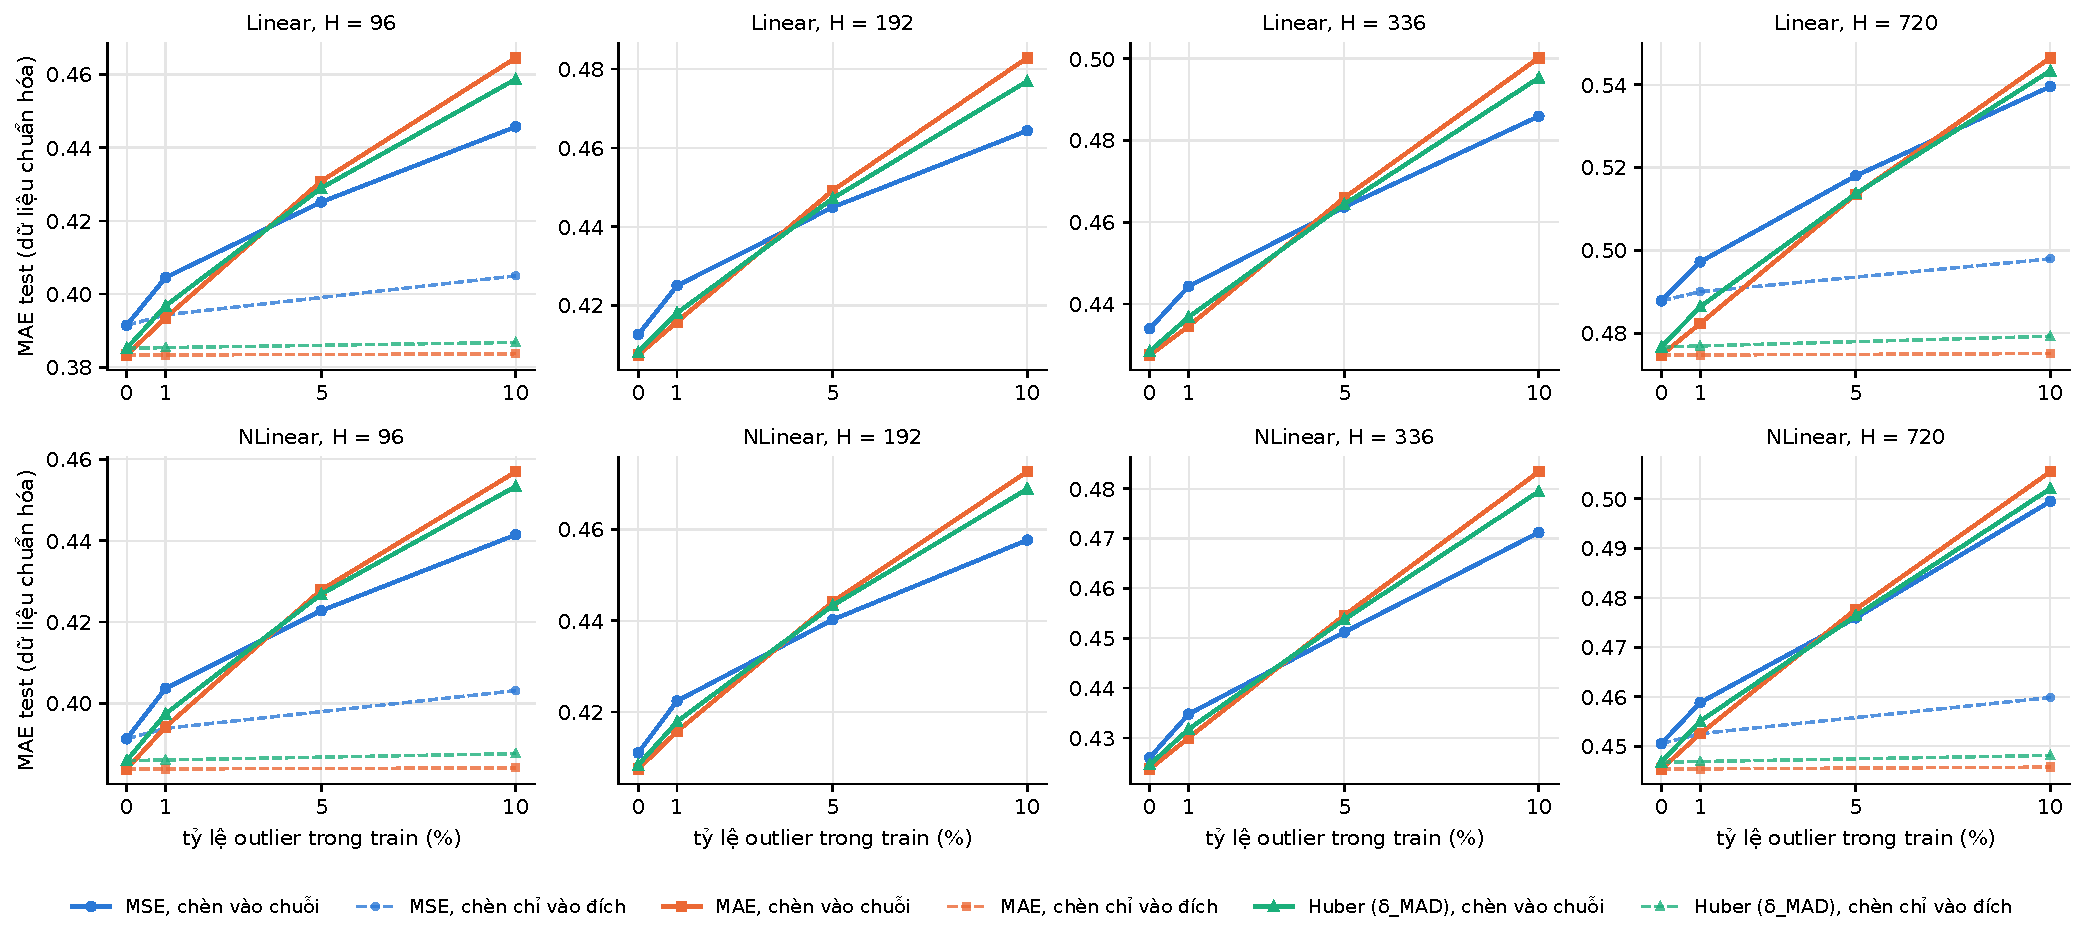
\includegraphics[width=\linewidth]{H2_outlier_mae.pdf}
\begin{figurecardcaptionaivn}
\capfig{Như \figref{fig:h2} nhưng là MAE test ở $\lambda^*_{\mathrm{MAE}}$ (chọn theo MAE val sạch).}\label{fig:h2mae}
\end{figurecardcaptionaivn}
\end{figure}

\begin{center}
\small
% Tự động sinh bởi scripts/report/make_tables.py từ results/. KHÔNG SỬA TAY.
\begin{tabular}{@{}r l r r rrr rrr@{}}
\toprule
 & & & & \multicolumn{3}{c}{MSE test ở $\lambda^*_{\mathrm{MSE}}$} & \multicolumn{3}{c}{MAE test ở $\lambda^*_{\mathrm{MAE}}$} \\
\cmidrule(lr){5-7}\cmidrule(l){8-10}
$H$ & chèn & tỷ lệ & độ lớn & MSE & MAE & Huber & MSE & MAE & Huber \\
\midrule
96 & gốc & -- & -- & 0{,}3702 & \textbf{0{,}3653} & 0{,}3658 & 0{,}3915 & \textbf{0{,}3833} & 0{,}3852 \\
96 & chuỗi & 1\% & 3$\sigma$ & 0{,}3700 & \textbf{0{,}3622} & 0{,}3643 & 0{,}3924 & \textbf{0{,}3831} & 0{,}3857 \\
96 & chuỗi & 1\% & 5$\sigma$ & 0{,}3720 & \textbf{0{,}3620} & 0{,}3650 & 0{,}3952 & \textbf{0{,}3851} & 0{,}3880 \\
96 & chuỗi & 1\% & 10$\sigma$ & 0{,}3818 & \textbf{0{,}3688} & 0{,}3731 & 0{,}4045 & \textbf{0{,}3935} & 0{,}3968 \\
96 & chuỗi & 10\% & 3$\sigma$ & 0{,}3799 & \textbf{0{,}3745} & 0{,}3757 & 0{,}4026 & \textbf{0{,}3979} & 0{,}3990 \\
96 & chuỗi & 10\% & 5$\sigma$ & \textbf{0{,}3954} & 0{,}3969 & 0{,}3958 & 0{,}4144 & 0{,}4144 & \textbf{0{,}4138} \\
96 & chuỗi & 10\% & 10$\sigma$ & \textbf{0{,}4445} & 0{,}4790 & 0{,}4691 & \textbf{0{,}4457} & 0{,}4645 & 0{,}4587 \\
96 & đích & 1\% & 3$\sigma$ & 0{,}3705 & \textbf{0{,}3654} & 0{,}3659 & 0{,}3918 & \textbf{0{,}3834} & 0{,}3853 \\
96 & đích & 1\% & 5$\sigma$ & 0{,}3709 & \textbf{0{,}3654} & 0{,}3659 & 0{,}3924 & \textbf{0{,}3834} & 0{,}3853 \\
96 & đích & 1\% & 10$\sigma$ & 0{,}3727 & \textbf{0{,}3654} & 0{,}3659 & 0{,}3943 & \textbf{0{,}3834} & 0{,}3854 \\
96 & đích & 10\% & 3$\sigma$ & 0{,}3721 & \textbf{0{,}3651} & 0{,}3667 & 0{,}3939 & \textbf{0{,}3836} & 0{,}3862 \\
96 & đích & 10\% & 5$\sigma$ & 0{,}3750 & \textbf{0{,}3651} & 0{,}3668 & 0{,}3967 & \textbf{0{,}3837} & 0{,}3863 \\
96 & đích & 10\% & 10$\sigma$ & 0{,}3841 & \textbf{0{,}3651} & 0{,}3667 & 0{,}4050 & \textbf{0{,}3837} & 0{,}3868 \\
\midrule
720 & gốc & -- & -- & 0{,}4701 & \textbf{0{,}4553} & 0{,}4624 & 0{,}4878 & \textbf{0{,}4747} & 0{,}4767 \\
720 & chuỗi & 1\% & 3$\sigma$ & 0{,}4704 & \textbf{0{,}4566} & 0{,}4573 & 0{,}4887 & \textbf{0{,}4757} & 0{,}4772 \\
720 & chuỗi & 1\% & 5$\sigma$ & 0{,}4712 & \textbf{0{,}4584} & 0{,}4589 & 0{,}4902 & \textbf{0{,}4746} & 0{,}4786 \\
720 & chuỗi & 1\% & 10$\sigma$ & 0{,}4765 & \textbf{0{,}4578} & 0{,}4629 & 0{,}4972 & \textbf{0{,}4824} & 0{,}4864 \\
720 & chuỗi & 10\% & 3$\sigma$ & 0{,}4757 & \textbf{0{,}4627} & 0{,}4644 & 0{,}4957 & \textbf{0{,}4844} & 0{,}4876 \\
720 & chuỗi & 10\% & 5$\sigma$ & 0{,}4904 & \textbf{0{,}4814} & 0{,}4830 & 0{,}5065 & \textbf{0{,}5004} & 0{,}5014 \\
720 & chuỗi & 10\% & 10$\sigma$ & \textbf{0{,}5470} & 0{,}5597 & 0{,}5527 & \textbf{0{,}5396} & 0{,}5465 & 0{,}5433 \\
720 & đích & 1\% & 3$\sigma$ & 0{,}4702 & \textbf{0{,}4554} & 0{,}4628 & 0{,}4881 & \textbf{0{,}4748} & 0{,}4769 \\
720 & đích & 1\% & 5$\sigma$ & 0{,}4706 & \textbf{0{,}4554} & 0{,}4628 & 0{,}4885 & \textbf{0{,}4748} & 0{,}4769 \\
720 & đích & 1\% & 10$\sigma$ & 0{,}4716 & \textbf{0{,}4554} & 0{,}4629 & 0{,}4900 & \textbf{0{,}4748} & 0{,}4769 \\
720 & đích & 10\% & 3$\sigma$ & 0{,}4714 & \textbf{0{,}4562} & 0{,}4584 & 0{,}4898 & \textbf{0{,}4751} & 0{,}4784 \\
720 & đích & 10\% & 5$\sigma$ & 0{,}4734 & \textbf{0{,}4562} & 0{,}4586 & 0{,}4919 & \textbf{0{,}4751} & 0{,}4785 \\
720 & đích & 10\% & 10$\sigma$ & 0{,}4798 & \textbf{0{,}4562} & 0{,}4596 & 0{,}4980 & \textbf{0{,}4751} & 0{,}4793 \\
\bottomrule
\end{tabular}

\end{center}
\begin{captionbelowboxaivn}
\captab{Độ lớn outlier: Linear, ETTh1, seed 2026, cùng vị trí outlier ở mọi độ lớn. \textbf{Đậm}: thấp nhất giữa ba mục tiêu.}\label{tab:magnitude}
\end{captionbelowboxaivn}
